\documentclass{beamer}
\useoutertheme[subsection=false]{miniframes}
\useinnertheme{rounded}
\usecolortheme{orchid}
\usecolortheme{whale}
\setbeamercolor{section in head/foot}{bg=white, fg=black}

\title{Predictive Maintenance for Industrial Machines}
\subtitle{Machine Learning 1 -- Final Project}
\author{Kayra Soykara \& Julian Oehler}
\institute{PSAI - PSL University}
\date{June 19, 2026}

\begin{document}

    \begin{frame}
        \titlepage
    \end{frame}

    \section{Introduction}

    \begin{frame}
        \frametitle{Objectives}
        \begin{itemize}
            \item Provide maintenance decisions for FactoryPulse machines
            \item Establish a policy for FactoryPulse to react to the maintenance decision
        \end{itemize}
    \end{frame}

    \begin{frame}
        \frametitle{Initial Exploratory Insights}
        \begin{itemize}
            \item Machine failures only occur in a small proportion of the data.
            \item Features regarding machine age, operating hours, vibration measures and prior failures are the most
            impactful on failure.
        \end{itemize}
    \end{frame}

    \begin{frame}
        \frametitle{Vibration Analysis}
        \centering
        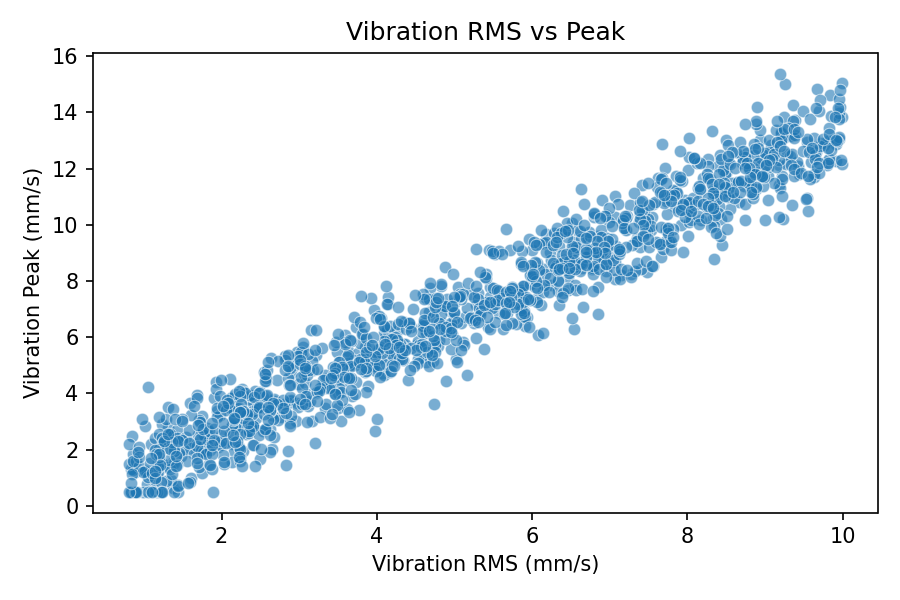
\includegraphics[width=0.75\textwidth]{img/vibration_scatter.png}
        \vspace{0.5em}

        The two vibration features are strongly related, which may introduce some redundancy.

    \end{frame}

    \section{Modeling}

    \begin{frame}
        \frametitle{}
    \end{frame}

\end{document}

